%
% db-normalverteilung.tex -- datenblatt der Normalverteilung
%
% (c) 2015 Prof Dr Andreas Mueller, Hochschule Rapperswil
%
\subsection{Steckbrief}
\begin{center}
\renewcommand{\arraystretch}{2}
\begin{tabular}{|l|l|}
\hline
Name&Normalverteilung\\
\hline
\setlength{\extrarowheight}{2pt}
Dichtefunktion&$\displaystyle\frac{1}{\sqrt{2\pi}\sigma}e^{-\frac{(x-\mu)^2}{2\sigma^2}}$\\
Verteilungsfunktion&keine elementare Funktion\\
Erwartungswert&$\mu$\\
Varianz&$\sigma^2$\\
Median&$\mu$\\
$P(|X-E(X)|>\varepsilon)$&keine einfache Formel\\
\hline
%\setlength{\extrarowheight}{50pt}
Anwendungen&
\begin{minipage}{3.7in}%
\vskip4pt
\strut
$\bullet$ Messwerte\\
$\bullet$ Summe vieler kleiner Einflüsse vergleichbar grosser Varianz
(Zentraler Grenzwertsatz)
\\
$\bullet$ Approximation der Binomialverteilung
\strut
\end{minipage}\\[21pt]
\hline
\end{tabular}
\end{center}

\subsection{Verteilungsfunktion und Wahrscheinlichkeitsdichte}
Verteilungsfunktion (oben) und Dichtefunktion (unten) der Normalverteilung:
\begin{center}
%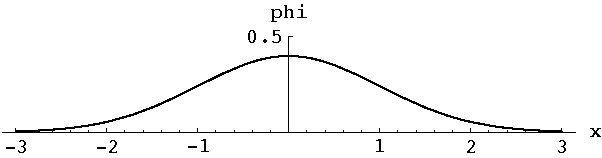
\includegraphics[width=0.8\hsize]{graphics/normphi}
%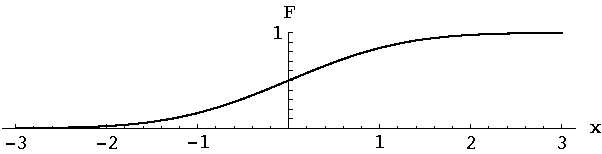
\includegraphics[width=0.8\hsize]{graphics/normF}
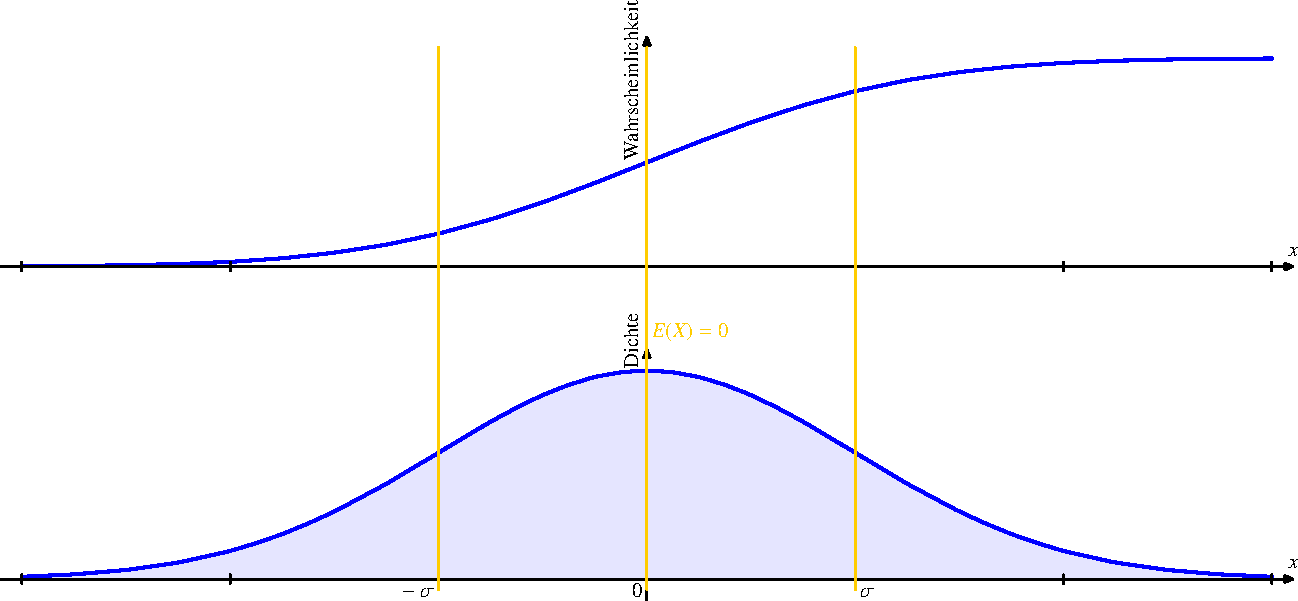
\includegraphics[width=\hsize]{images/verteilungsfunktion-9}
\end{center}

\subsection{Wahrscheinlichkeit einer grossen Abweichung}
Vergleich der Wahrscheinlichkeit für eine grosse Abweichung
für die Normalverteilung (rot) und die Schranke von Tschebyscheff (grün):
\begin{center}
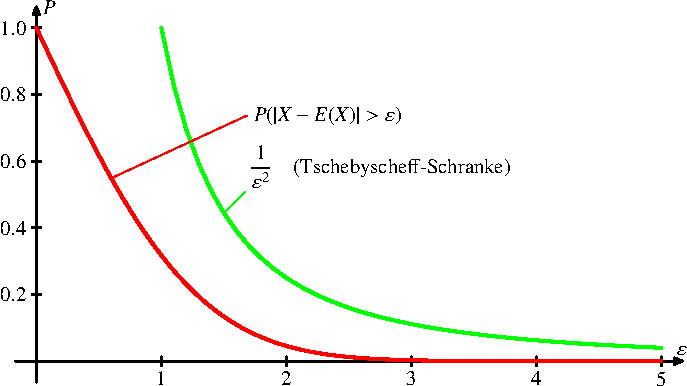
\includegraphics{images/norm-1.pdf}
\end{center}

\subsection{Parameter schätzen}
Die Parameter $\mu$ und $\sigma$ können mit den erwartungstreuen Schätzern
\begin{align*}
\hat\mu(x_1,\dots,x_n)&=\frac{x_1+\dots+x_n}{n}\\
\hat\sigma(x_1,\dots,x_n)^2&=\frac{1}{n-1}\biggl(
\sum_{i=1}^n x_i^2 - \frac1n\biggl(\sum_{i=1}^n x_i\biggr)^2
\biggr)
\end{align*}
geschätzt werden.

Der Mittelwert ist $\hat\mu(x_1,\dots,x_n)$ ist normalverteilt mit Erwartungswert
$\mu$ und Varianz $\frac1n\sigma^2$.
Die Stichprobenvarianz $\hat\sigma(x_1,\dots,x_n)^2/\sigma^2$ ist $\chi^2$-verteilt
mit $n-1$ Freiheitsgraden.

\subsection{Zentraler Grenzwertsatz}
Der zentrale Grenzwertsatz besagt, dass die Verteilungsfunktion einer Summe
einer grossen Zahl von Zufallsvariablen unter milden Voraussetzungen
gegen die Verteilungsfunktion einer Normalverteilung konvergiert.
Dies rechtfertigt den Einsatz der Normalverteilung als Modell für Prozesse,
in denen eine grosse Zahl von vergleichbar grossen Einflüssen zu einem Effekt
beitragen, zum Beispiel bei Messwerten.

\subsection{Standardisierung}
Ist $X$ eine normalverteilte Zufallsvariable, dann ist 
\[
Z=\frac{X-\mu}{\sigma}
\]
eine normalverteilte Zufallsvariable mit Erwartungswert $0$ und Varianz $1$,
d.~h.~eine standardnormalverteilte Zufallsvariable.
Für die Standardnormalverteilung ist im Tabellenanhang eine Tabelle der
Verteilungsfunktion sowie einzelner Quantilen zu finden.

Man beachte, dass die Zufallsvariable $Z$ nicht mehr normalverteilt ist, wenn man
$\mu$ und $\sigma$ durch Schätzwerte ersetzt, die resultierende Verteilung
ist dann eine $t$-Verteilung.
